%%%%%%%%%%%%%%%%%%%%%%%%%%%%%%%%%%%%%%%%%
% University/School Laboratory Report
% LaTeX Template
% Version 3.1 (25/3/14)
%
% This template has been downloaded from:
% http://www.LaTeXTemplates.com
%
% Original author:
% Linux and Unix Users Group at Virginia Tech Wiki 
% (https://vtluug.org/wiki/Example_LaTeX_chem_lab_report)
%
% License:
% CC BY-NC-SA 3.0 (http://creativecommons.org/licenses/by-nc-sa/3.0/)
%
%%%%%%%%%%%%%%%%%%%%%%%%%%%%%%%%%%%%%%%%%

%----------------------------------------------------------------------------------------
%	PACKAGES AND DOCUMENT CONFIGURATIONS
%----------------------------------------------------------------------------------------

\documentclass{article}

\usepackage{graphicx} % Required for the inclusion of images
\usepackage{amsmath} % Required for some math elements
\usepackage{enumitem}

\setlength\parindent{0pt} % Removes all indentation from paragraphs

\renewcommand{\labelenumi}{\alph{enumi}.} % Make numbering in the enumerate environment by letter rather than number (e.g. section 6)

\newlist{inlinelist}{enumerate*}{1}
\setlist*[inlinelist,1]{%
  label=(\arabic*),
}

%----------------------------------------------------------------------------------------
%	DOCUMENT INFORMATION
%----------------------------------------------------------------------------------------

\title{\begin{LARGE}
	\textbf{EE 445L - Lab 3: Alarm Clock}
\end{LARGE}} % Title

\author{Joshua Bryant \\ jmb6357 \and James Morris \\ jsm3288} % Author name

\date{\today} % Date for the report

\begin{document}

\maketitle % Insert the title, author and date

%----------------------------------------------------------------------------------------
%	SECTION 1 Objectives
%----------------------------------------------------------------------------------------

\section{Objective}

	\subsection{Overview}

		\subsubsection{Objectives}
		The objectives of this project are to design, build, and test an alarm clock. Educationally, students are learning how to design and test modular software and how to perform switch/keypad input in the background.

		\subsubsection{Process}
		The project will be developed using the TM4C123 board. There will be switches or a keypad. The system will be built on a solderless breadboard and run on the usual USB power. The system may use the on board switches and/or the on board sound. Alternatively, the system may include an external keypad and/or speaker. There will be at least four hardware/software modules: switch/keypad input, time management, OLED graphics, and sound output. The process will be to design and test each module independently from the other modules. After each module is tested, the system will be built and tested.
	
		\subsubsection{Roles and Responsibilities}
		EE445L students are the engineers and the TA is the client. Students are expected to modify this document to clarify exactly what they plan to build. Students are allowed to divide responsibilities of the project however they wish, but, at the time of demonstration, both students are expected to understand all aspects of the design.
	
		\subsubsection{Interactions with Existing Systems}
		The system will use the TM4C123 board, a ST7735 color LCD, a solderless breadboard, and be powered using the USB cable.	
	
		\subsubsection{Terminology}
			\begin{description}
				\item[Power Budget]
					An estimation of the operation time of a battery-powered embedded system by obtained by dividing the energy storage by the average current required to run the system.
				
				\item[Device Driver]
					A collection of software routines that perform I/O functions.			
			
				\item[Critical Section]
					Locations within a software module, which if an interrupt were to occur at one of these locations, then an error could occur (e.g., data lost, corrupted data, program crash, etc.) Same as vulnerable window.
				
				\item[Latency]
					The response time of the computer to external events. Can also be used in reference to I/O devices, which is the response time of the external I/O device hardware to a software command.
			
				\item[Time Jitter]
					Deviation in the time domain of intended signal value, often encountered at fast shifts between different voltage levels.
			
				\item[Modular Programming]
					A style of software development that divides the software problem into distinct and independent modules. The parts are as small as possible, yet relatively independent. 
			
			\end{description}
	
		\subsubsection{Security}
		The system may include software from Tivaware and from the book. No software written for this project may be transmitted, viewed, or communicated with any other EE445L student past, present, or future. It is the responsibility of the team to keep its EE445L lab solutions secure.

	\subsection{Function Description}

		\subsubsection{Functionality}
			The clock must be able to perform five functions:
			\begin{enumerate}
				\item
					It will display hours, minutes, and seconds in both graphical and numeric forms on the LCD. The graphical output will include the 12 numbers around a circle, the hour hand, and the minute hand. The numerical output will be easy to read.
			
				\item
					It will allow the operator to set the current time using switches or a keypad. The user will also be able to switch between 12 and 24 hour time representations.
				
				\item
					It will allow the operator to set the alarm time including enabling/disabling alarms.
				
				\item
					It will allow the operator to stop the sound.				
			\end{enumerate}
			An LED heartbeat will show when the system is running.
	
		\subsubsection{Scope}
			Phase 1 is the preparation; phase 2 is the demonstration; and phase 3 is the lab report. Details can be found in the lab manual.
	
		\subsubsection{Prototypes}
			A prototype system running on the TM4C123 board, ST7735 color LCD, and solderless breadboard will be demonstrated. Progress will be judged by the preparations, demonstration, and lab report.
	
		\subsubsection{Performance}
			The system will be judged by three qualitative measures. First, the software modules must be easy to understand and well-organized. Second, the clock display should be beautiful and effective in telling time. Third, the operation of setting the time and alarm should be simple and intuitive. The system should not have critical sections. All shared global variables must be identified with documentation that a critical section does not exist. Backward jumps in the ISR should be avoided if possible. The interrupt service routine used to maintain time must complete in as short a time as possible. This means all LCD I/O occurs in the main program. The average current on the +5V power will be measured with and without the alarm sounding.
	
		\subsubsection{Usability}
			There will be five switch inputs. In the main menu, the switches can be used to activate
			\begin{inlinelist}
				\item set time
				\item set alarm
				\item alarm on\textbackslash off
				\item 12\textbackslash 24 hour mode
				\item display mode
			\end{inlinelist}.
			In the set time and alarm modes, two switches add and subtract hours and the other two add and subtract minutes. After 10 seconds of inactivity the system reverts to the main menu. The 12\textbackslash 24 hour mode switch toggles between 12 and 24 hour time representations. The display mode switch toggles between graphical and numeric displays. The switches will be debounced, so only one action occurs when the operator touches a switch once.\\
			The LCD display shows the time using graphical display typical of a standard on the wall clock. The 12 numbers, the second hand, the minute hand, and the hour hand are large and easy to see. The clock can also display the time in numeric mode using numbers.\\
			The alarm sound can be a simple square wave. The sound amplitude will be just loud enough for the TA to hear when within 3 feet.
		
		\subsubsection{Safety}
			The alarm sound will be very quiet in order to respect other people in the room during testing. Connecting or disconnecting wires on the protoboard while power is applied may damage the board.

	\subsection{Deliverables}

		\subsubsection{Reports}
			A lab report described below is due by the due date listed in the syllabus. This report includes the final requirements document.
	
		\subsubsection{Audits}
			The preparation is due at the beginning of the lab period on the date listed in the syllabus.
	
		\subsubsection{Outcomes}
			There are three deliverables:
			\begin{inlinelist}
				\item preparation
				\item demonstration
				\item report
			\end{inlinelist}.

 
%----------------------------------------------------------------------------------------
%	SECTION 2 Hardware Design
%----------------------------------------------------------------------------------------
\section{Hardware Design}
	\begin{figure}[h]
		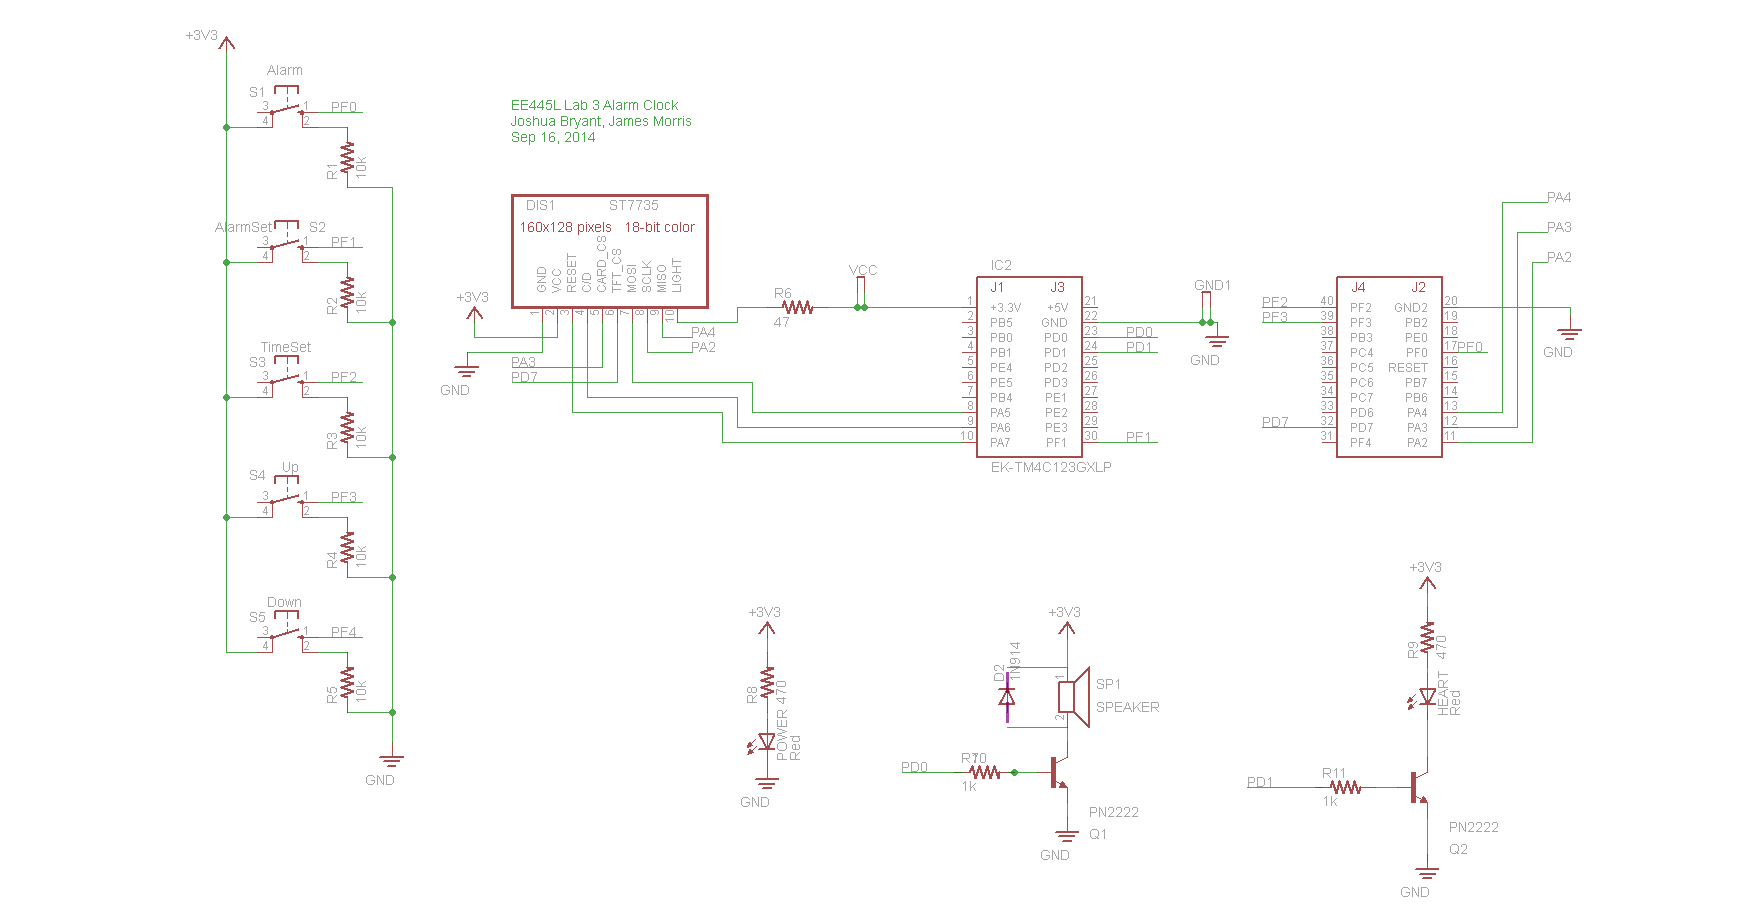
\includegraphics[keepaspectratio, width=\textwidth]{Lab3Graphics/Schematic.png}
		\caption{Schematic showing connection of all external components connected to the TM4C123}
		\label{fig:schematic}
	\end{figure}

%----------------------------------------------------------------------------------------
%	SECTION 3 Software Design
%----------------------------------------------------------------------------------------
%\section{Software Design} %not needed for this lab. Just submit code to Canvas

%----------------------------------------------------------------------------------------
%	SECTION 4 Measurement Data
%----------------------------------------------------------------------------------------
%\section{Measurement Data} %include when you actually have screen shots for the lab report

%----------------------------------------------------------------------------------------
%	SECTION 5 Analysis and Discussion
%----------------------------------------------------------------------------------------
\section{Analysis and Discussion}

	\begin{enumerate}
		\item %Qustion 1
			One way to remove a critical section is to remove read-modify-write sections of code accessing a shared global variable. Another method of removing critical sections is to disable interrupts before accessing the variable and re-enable interrupts after writing to the variable.
			
		\item %Question 2
			It takes approximately 20ms to update the LCD with a new time.
					
		\item %Question 3
			A disadvantage of updating the LCD in the background ISR is that updating the screen takes a relatively long period of time and can cause error in the timing to occur if the timing interrupt is not allowed to interrupt the screen update ISR.
		
		\item %Question 4
			No, we did not redraw the entire clock for each output. We only redrew the minute, second, and hour hand for each output to reduce the amount of time needed to redraw the screen resulting in a faster update rate and less flicker on the screen.
						
		\item %Question 5
			The following is a list of some of the ways we could have saved power if the system was battery powered:
			\begin{inlinelist}
				\item reducing the screen brightness
				\item reducing the speaker volume through a larger resistor to the transistor and
				\item switching the switches to connect to ground and only connect to power when being pressed
			\end{inlinelist}.
	\end{enumerate}

\end{document}